%form: dc_form_05-07.tex ; user: dc_05-07_purpose_plan_rights.tex
%========== DC =========
%===== p. 05-07 研究の目的・内容、特色、計画、人権 =============
\subsection{研究の目的・内容}
%watermark: w02_purpose_plan_ugly_dc
\newcommand{\研究目的}{%
%begin  研究目的と内容===================
	象の卵の研究の目的は...
%end  研究目的と内容 ====================
}

\newcommand{\人権の保護及び法令等の遵守への対応}{%
%begin  人権の保護及び法令等の遵守への対応 ===================
	象の卵のES細胞の培養、象のクローンの生成などは行わない。
	象個体を現地から持ち出すことはないので、ワシントン条約ならびに
        生物多様性条約に抵触しない。また、組換え実験は行なわないので、
        カルタヘナ議定書にも抵触しない。
%end  人権の保護及び法令等の遵守への対応 ====================
}

\newcommand{\研究の特色と独創的な点tillNextPage}{%
%begin  研究の特色と独創的な点===================
	今まで、研究者は皆「ほ乳類は卵を産まない」という生物学のいわゆる「常識」に
	捕われ、象が卵を産むなどということはあり得ないと考えていた。
	しかし、ほ乳類は文字通り、産まれた乳幼児に乳を与える動物の総称であり、
	産まれる過程を規定しているわけではない。
	象のように大きな動物にあっては、体内に大きな胎児をかかえて移動するよりは、
	卵を産んでそれを暖め、ふ化してから乳を与えて育てる方が効率的である。
	
	したがって、今までの「常識」を打ち砕く新たな観点が、この研究の独創的な点である。

	とにかく何か書いて文字数をかせいで、次のページまで流れ込むようにしよう。
	とにかく何か書いて文字数をかせいで、次のページまで流れ込むようにしよう。
	とにかく何か書いて文字数をかせいで、次のページまで流れ込むようにしよう。
	とにかく何か書いて文字数をかせいで、次のページまで流れ込むようにしよう。
	とにかく何か書いて文字数をかせいで、次のページまで流れ込むようにしよう。
	とにかく何か書いて文字数をかせいで、次のページまで流れ込むようにしよう。
	とにかく何か書いて文字数をかせいで、次のページまで流れ込むようにしよう。
	とにかく何か書いて文字数をかせいで、次のページまで流れ込むようにしよう。
	とにかく何か書いて文字数をかせいで、次のページまで流れ込むようにしよう。
	とにかく何か書いて文字数をかせいで、次のページまで流れ込むようにしよう。
	とにかく何か書いて文字数をかせいで、次のページまで流れ込むようにしよう。
	とにかく何か書いて文字数をかせいで、次のページまで流れ込むようにしよう。
	とにかく何か書いて文字数をかせいで、次のページまで流れ込むようにしよう。
	とにかく何か書いて文字数をかせいで、次のページまで流れ込むようにしよう。
	とにかく何か書いて文字数をかせいで、次のページまで流れ込むようにしよう。
	とにかく何か書いて文字数をかせいで、次のページまで流れ込むようにしよう。
	とにかく何か書いて文字数をかせいで、次のページまで流れ込むようにしよう。
%end  研究の特色と独創的な点 ====================
}

\newcommand{\研究計画withVspaceDC}{%
%begin  研究計画 ===================
	% 今年の様式は困ったものです。ブツブツ。
	% 今の技術では「(4)研究計画」のスタート位置を指定できることができません。
	% すみませんが、次の2行を調整してください。
%	\clearpage	% もし「(3) 研究の特色・独創的な点」がp.6に流れこまないなら、この行を有効にしてください。
	\vspace*{110mm}	% 「(4) 研究計画」が正しい高さから始まるように、この値を調整してください。

\textbf{この行の高さは、上の「研究の特色・独創的な点」との間隔を\textbackslash vspaceを用いて調整してください。}

        \begin{figure}[h]
         	\begin{minipage}[t]{0.49\linewidth}
			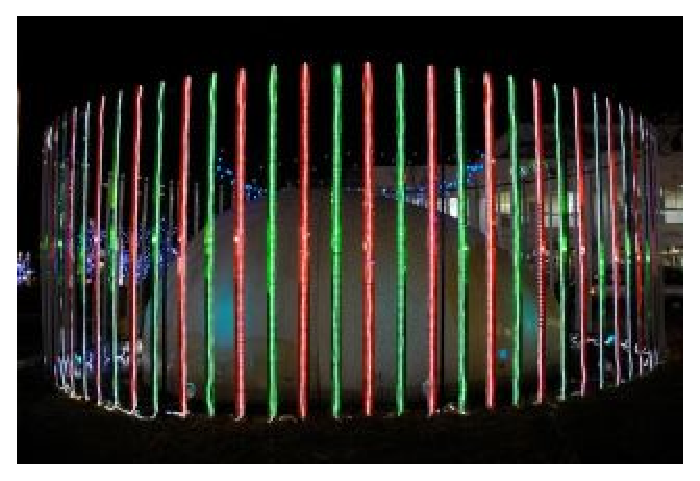
\includegraphics[width=\linewidth]{figs/egg_R.eps}
			\caption{右目用}
			\label{fig:egg_R}
		\end{minipage}
		\hspace{0.01\linewidth}
		\begin{minipage}[t]{0.49\linewidth}
			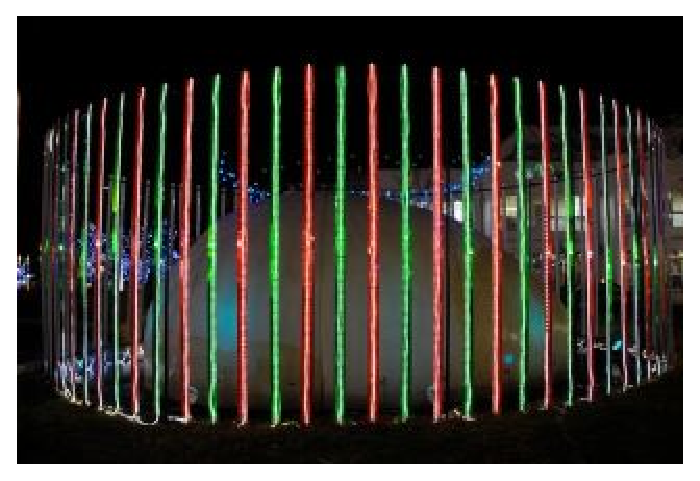
\includegraphics[width=\linewidth]{figs/egg_L.eps}
			\caption{左目用}
			\label{fig:egg_L}
		\end{minipage}
         \end{figure}
	実はこの象の卵の像の中に本当の卵が隠されている可能性もあるため、
	最新の技術を用いて非破壊的に内部を調査する。

	象の卵の研究の計画と方法は...
%end  研究計画 ====================
}

